
\section{О ПРОПУСКНОЙ СПОСОБНОСТИ «ЭФИРА» И ПРОВОЛОКИ В ЭЛЕКТРОСВЯЗИ}

\textbf{Автор:} Безянова Елизавета Юрьевна, Б-01-009

Как в радио-, так и в проволочной технике для каждой передачи требуется не одна какая-либо частота, а целый диапазон частот. Это ведет к тому, что одновременно может работать лишь ограниченное количество радиостанций (передающих разные программы). По одной паре проводов также нельзя передавать сразу больше определенного количества передач, так как нельзя, чтобы полоса частот одной передачи перекрывала полосу другой, --- такое перекрытие привело бы к взаимным помехам.

Чтобы увеличить пропускную способность «эфира» и проволоки (а это имело бы колоссальное практическое значение, в особенности в связи с бурным развитием радиотехники и таких передач, как телевидение), нужно как-то сократить диапазон частот, требуемый для данной передачи, не вредя ее качеству, или изобрести способ разделения передач не по частотному признаку, как это делалось до сих пор, а по какому-нибудь другому.

По настоящее время никакие ухищрения в этих направлениях не позволяли, даже теоретически, увеличить пропускную способность «эфира» и проволоки в большей степени, чем это позволяет сделать передача «на одной боковой полосе».

Поэтому возникает вопрос: возможно ли вообще это сделать? Или же все попытки в этом направлении будут равносильны попыткам построить perpetuum mobile?

Этот вопрос в настоящее время имеет актуальное значение в радиотехнике ввиду с каждым годом все увеличивающейся «тесноты в эфире». И сейчас особенно важно в нем разобраться в связи с планированием научно-исследовательских работ, так как при планировании важно знать, что возможно и что совершенно невозможно сделать, чтобы направить силы в нужном направлении.

В настоящей работе разбирается этот вопрос и доказывается, что для телевидения и передачи изображений со всеми полутенями, а также для телефонной передачи существует вполне определенная, минимально необходимая полоса частот, которую, не вредя качеству передачи и скорости, нельзя никакими средствами уменьшить; а также доказывается, что для этих передач нельзя увеличить пропускную способность ни эфира, ни проволоки путем применения разного рода нечастотных селекций или других каких-либо способов (исключая, конечно, селекцию по направлению при помощи направленных антенн). Максимально возможная пропускная способность для этих передач может быть получена при передаче «на одной боковой полосе», и она является в настоящее время принципиально вполне достижимой.

Для таких же передач, как телеграфия или же передача изображений и телевидения без полутеней и т. п., в которых передаваемый объект может меняться не непрерывно, а принимая лишь определенные, наперед известные значения, показывается, что необходимая для них полоса частот может быть уменьшена во сколько угодно раз, не вредя ни качеству передачи, ни скорости, за счет увеличения мощности и усложнения аппаратуры. Один из методов такого уменьшения полосы частот указывается в этой работе и показывается, какое увеличение мощности для этого необходимо.

Таким образом, предела для пропускной способности «эфира» и проволоки для передач такого вида теоретически не имеется, дело лишь в техническом выполнении.

Доказательство этих положений в этой работе ведется вне зависимости от метода передачи на основании следующего: во всех видах электросвязи передатчик может передавать, а приемник принимать лишь некоторую функцию времени, которая не может быть вполне произвольной, так как частоты, из которых она состоит и на которые она может быть разложена, должны заключаться в определенных пределах. При радиопередаче такой функцией является сила тока в передающей антенне, которая и воспринимается приемником более или менее точно; при проволочной же передаче это будет электродвижущая сила в начале линии. В обоих случаях передаваемые функции будут состоять из частот ограниченного диапазона, так как, во-первых, очень высокие и очень низкие частоты не дойдут до приемника по условиям распространения, и, во-вторых, частоты, выходящие за пределы определенного узкого диапазона, обычно нарочно уничтожаются, чтобы не мешать другим передачам.

Эта необходимость передавать при помощи функций времени, состоящих из ограниченного диапазона частот, уже приводнт, как это будет ниже показано, к вполне определенному ограничению пропускной способности.

Для доказательства высказанных положений займемся изучением функций, состоящих из определенного диапазона частот.\newline

\subsection*{Функции, состоящие из частот от 0 до $f_1$} 

\begin{definition} Пусть $2\pi$-периодическая функция $f \in L_R(-\pi,\pi)$. Тогда функция называется \textit{регулярной} $f$ в каждой точке $x$ в том случае, если она удовлетворяет равенству $$A = \frac{(f(x+0)+f(x-0))}{2}.$$
Далее мы будет рассматривать именно регулярные функции.
\end{definition}

\begin{theorem}\label{bezianova_theor_1} Любую функцию $F(t)$, состоящую из частот от 0 до $f_1$ периодов в секунду, можно представить рядом

\begin{equation}\label{bezianova_eq_1}
    F(t)=\sum_{-\infty}^{+\infty} D_k \frac{\sin \omega_1\left[t-k /\left(2 f_1\right)\right]}{t-k/\left(2 f_1\right)}, 
\end{equation}
где $k$ --- целое число; $\omega_1 = 2 \pi f_1 ; D_k$ --- постоянные, завнсящие от $F(t)$.

И наоборот, любая функция $F(t)$, представленная рядом $(\ref{bezianova_eq_1})$, состоит лишь из частот от 0 до $f_1$ периодов в секунду.

\end{theorem}

\begin{proof} Любая функция $F(t)$, удовлетворяющая условиям Дирихле (конечное число максимумов, минимумов и точек разрыва на любом конечном отрезке) и интегрируемая в пределах от $-\infty$ до $+\infty$, что всегда в электротехнике имеет место, может быть представлена интегралом Фурье
\begin{equation}\label{bezianova_eq_2}
    F(t)=\int_0^{\infty} C(\omega) \cos \omega t \text{ d} \omega+\int_0^{\infty} S(\omega) \sin \omega t \text{ d} \omega,
\end{equation}
т. е. как сумма бесконечного количества синусоидальных колебаний с частотами от 0 до $\infty$ и амплитудами $C(\omega) d \omega$ и $S(\omega) d \omega$, зависящими от частоты. Причем
\begin{equation} \label{bezianova_eq_3}
\begin{aligned}
& C(\omega)=\frac{1}{\pi} \int_{-\infty}^{+\infty} F(t) \cos \omega t \text{ d} t, \\
& S(\omega)=\frac{1}{\pi} \int_{-\infty}^{+\infty} F(t) \sin \omega t \text{ d} t.
\end{aligned}
\end{equation}

B нашем случае, когда $F(t)$ состоит лишь из частот от 0 до $f_1$, очевидно
$$
\begin{aligned}
& C(\omega)=0, \\
& S(\omega)=0
\end{aligned}
$$
при
$$
\omega>\omega_1=2 \pi f_1,
$$
и поэтому $F(t)$ может быть представлена согласно уравнению (\ref{bezianova_eq_2}) так:
\begin{equation}\label{bezianova_eq_4}
    F(t)=\int_0^{\omega_1} C(\omega) \cos \omega t \text{ d} \omega+\int_0^{\omega_1} S(\omega) \sin \omega t \text{ d} \omega.
\end{equation}
\qquad Функции же $C(\omega)$ и $S(\omega)$, как и всякие другие, на участке
$$
0<\omega<\omega_1
$$
могут быть представлены всегда рядами Фурье, причем эти ряды могут, по нашему желанию, состоять из одних косинусов или одних синусов, если мы возьмем за период двойную длину участка, т. е. $2 \omega_1$ ). Таким образом:


\begin{subequations}\label{bezianova_eq_5a}
\begin{align}
    C(\omega)=\sum_0^{\infty} A_k \cos \frac{2 \pi}{2 \omega_1} k \omega
    \end{align}
\end{subequations}
и
\begin{subequations}\label{bezianova_eq_5b}
\begin{align}
    S(\omega)=\sum_0^{\infty} B_k \sin \frac{2 \pi}{2 \omega_1} k \omega 
\end{align}
\end{subequations}


Введем следующие обозначения:
\begin{equation}\label{bezianova_eq_6}
\begin{gathered}
D_k=\frac{A_k+B_k}{2}, \\
D_{-k}=\frac{A_k-B_k}{2}, 
\end{gathered}
\end{equation}
тогда формулы (\ref{bezianova_eq_5a}) и (\ref{bezianova_eq_5b}) можно переписать так:
\begin{equation}\label{bezianova_eq_7}
\begin{aligned}
C(\omega) & =\sum_{-\infty}^{+\infty} D_k \cos \frac{\pi}{\omega_1} k \omega, \\
S(\omega) & =\sum_{-\infty}^{+\infty} D_k \sin \frac{\pi}{\omega_1} k \omega.
\end{aligned}
\end{equation}

Подставляя теперь выражения (\ref{bezianova_eq_7}) в формулу (\ref{bezianova_eq_4}), мы после некоторых преобразований и интегрирования (см. приложение I) получим уравнение (\ref{bezianova_eq_1}), т. е. докажем первую часть теоремы ~\ref{bezianova_theor_1}.

Для доказательства второй части теоремы рассмотрим частный случай $F(t)$, когда спектр частот, из которого она состоит, заключенв пределах от 0 до $f_1$ и выражается уравнениями (\ref{bezianova_eq_7}), в которых все $D_k$, кроме одного, равны нулю. Такая $F(t)$, очевидно, будет состоять из одного члена ряда (\ref{bezianova_eq_1}). Значит, и наоборот: если $F(t)$ состонт из одного, любого члена ряда (\ref{bezianova_eq_1}), то весь ее спектр заключен в пределах от 0 до $f_1$. А поэтому и сумма из любых отдельных членов ряда (\ref{bezianova_eq_1}), т. е. сам ряд (\ref{bezianova_eq_1}), будет состоять из частот, заключенных в пределах от 0 до $f_1$, что и требовалось доказать.

Все члены ряда (\ref{bezianova_eq_1}) подобны и отличаются лишь сдвигом по времени и множителями $D_k$. Один из членов, имеющий индекс $k$, изображен на рис.~\ref{fig::bezianova_pic_1} , он имеет максимум при $t=k /\left(2 f_1\right)$ и постепенно уменьшающуюся амплитуду в обе стороны.

\begin{figure}[H]
        \centering
        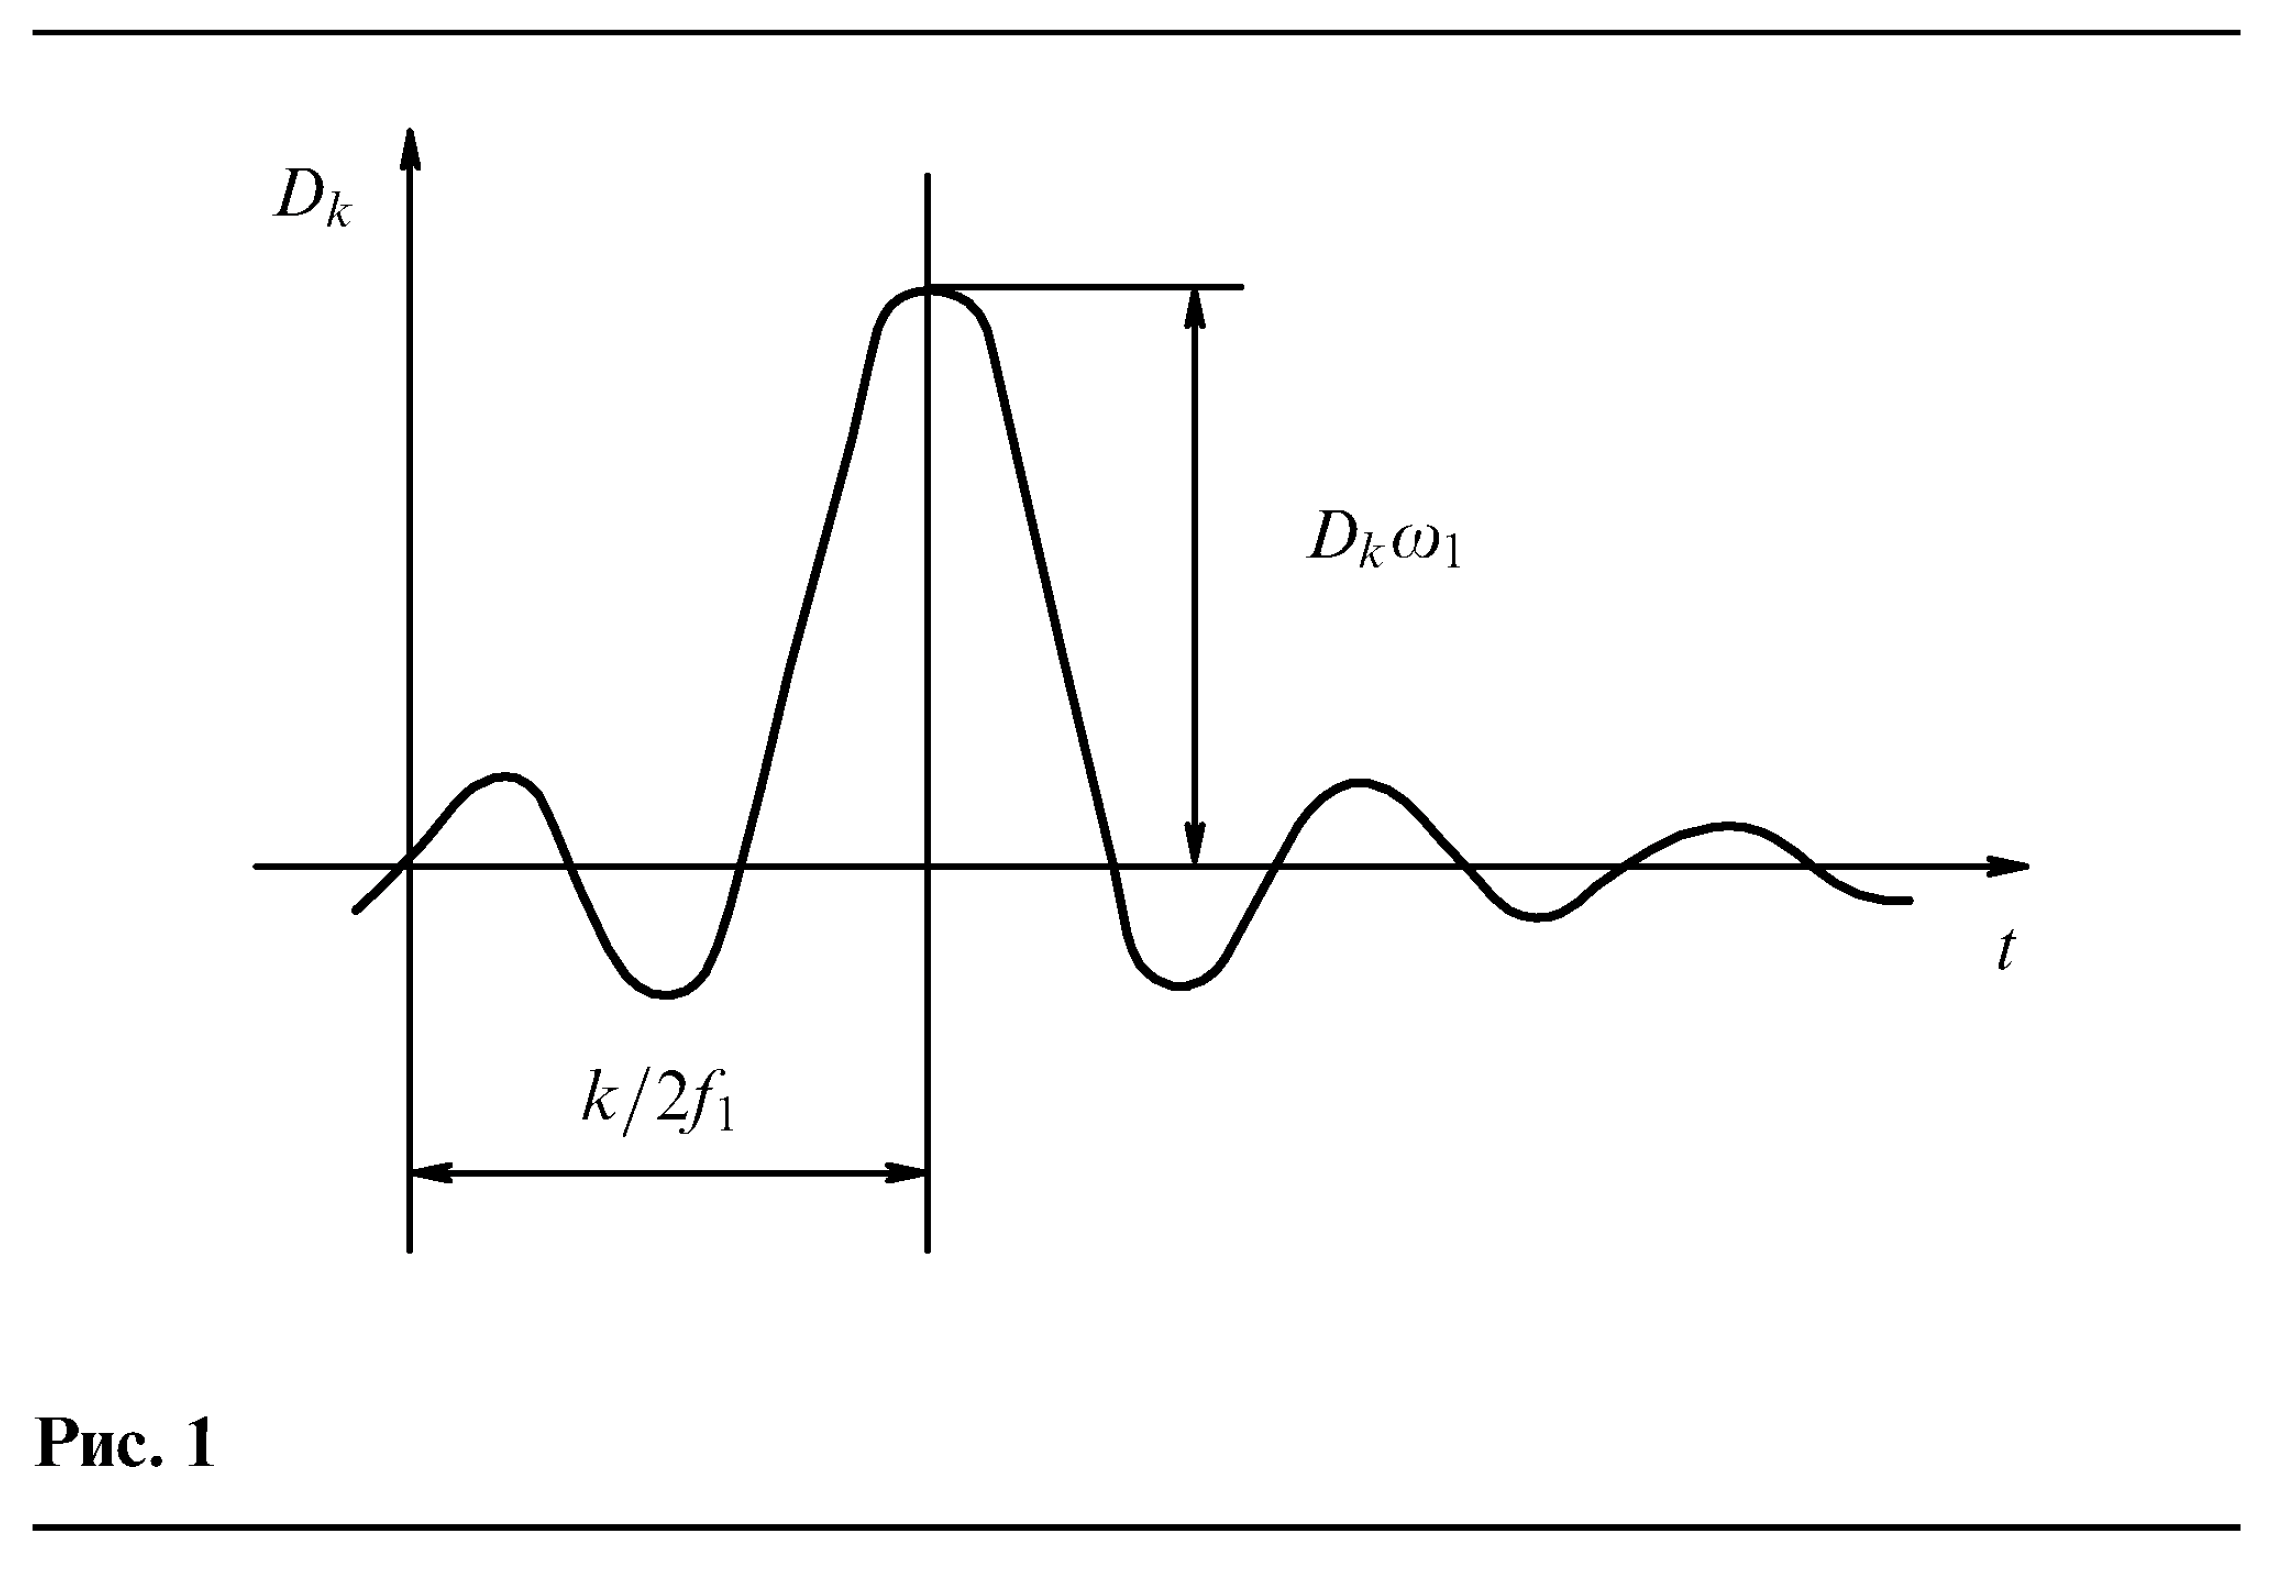
\includegraphics[width=0.7\linewidth]{bezianova_pic_1.png}
        \caption{~}
        \label{fig::bezianova_pic_1}
    \end{figure}
    
 \end{proof}
    
\begin{theorem}\label{bezianova_theor_2} Любую функцию $F(t)$, состоящую из частот от 0 до $f_1$, можно непрерывно передавать с любой точностью при помощи чисел, следующих друг за другом через $1 /\left(2 f_1\right)$ секунд. Действительно, измеряя величину $F(t)$ при $t=n /\left(2 f_1\right)(n-$ целое число), мы получим:
\begin{equation}\label{bezianova_eq_8}
F\left(\frac{n}{2 f_1}\right)=D_n \omega_1.
\end{equation}
\qquad Так как все члены ряда (\ref{bezianova_eq_1}) для этого значения $t$ обращаются в нули, кроме члена с $k=n$, который, как это легко можно получить, раскрывши неопределенность, будет равняться $D_n \omega_1$. Таким образом, через каждую $1/\left(2 f_1\right)$-ю секунду мы сможем узнавать очередное $D_k$. Передавая эти $D_k$ по очереди через каждые $1/\left(2f_1\right)$ секунд, мы сможем по ним согласно уравнению (\ref{bezianova_eq_1}) почленно восстановить $F(t)$ с любой точностью.
\end{theorem}

\begin{theorem}\label{bezianova_theor_3} Можно непрерывно и равномерно передавать произвольные числа $D_k$ со скоростью $N$ чисел в секунду при помощи функции $F(t)$, имеющей слагаемые на частотах больших $f_1=N / 2$ сколь угодно малыми.
	\end{theorem}

\begin{proof}
Действительно, будем по получению каждого числа строить функцию $F_k(t)$ такую, что
\begin{equation}\label{bezianova_eq_9}
\begin{aligned}
& \text { при } t<\frac{k}{2 f_1}-T \text{:} \quad F_k(t)=0, \\
& \text { при } \frac{k}{2 f_1}-T<t<\frac{k}{2 f_1}+T \text{:} 
\quad F_k(t)=D_k \frac{\sin \omega_1\left(t-k /\left(2 f_1\right)\right)}{t-k /\left(2 f_1\right)}, \\
& \text { при } t>\frac{k}{2 f_1}+T \text{:} \quad F_k(t)=0,
\end{aligned}
\end{equation}
и передавать их сумму $F(t)$. Если бы $T=\infty$, то полученная функция $F(t)$ состояла бы исключительно из частот меньших $f_1$, так как мы получили бы тогда ряд (\ref{bezianova_eq_1}), но, к сожалению, такие бесконечные ряды членов строить невозможно, поэтому будем ограничиваться конечными $T$. Докажем, что чем больше $T$, тем амплитуды на частотах $f>f_1$ будут становиться меньше и могут быть сделаны сколь угодно малыми. Для этого найдем амплитуды $C(\omega)$ и $S(\omega)$ для функции (\ref{bezianova_eq_9}) подстановкой ее в уравнение (\ref{bezianova_eq_3}). Получим:

\begin{equation}\label{bezianova_eq_10}
\begin{aligned}
& C(\omega)=\frac{1}{\pi} \int_{k /\left(2 f_1\right)-T}^{k /\left(2 f_1\right)+T} D_k \frac{\sin \omega_1\left(t-k /\left(2 f_1\right)\right)}{t-k /\left(2 f_1\right)} \cos \omega t \text{ d} t, \\
& S(\omega)=\frac{1}{\pi} \int_{k /\left(2 f_1\right)-T}^{k /\left(2 f_1\right)+T} D_k \frac{\sin \omega_1\left(t-k /\left(2 f_1\right)\right)}{t-k /\left(2 f_1\right)} \sin \omega t \text{ d} t .
\end{aligned}
\end{equation}

После интегрирования (см. приложение II) будем иметь
\begin{equation}\label{bezianova_eq_11}
\begin{aligned}
C(\omega) & =\frac{D_k}{\pi} \cos \omega \frac{k}{2 f_1}\left[\operatorname{Si} T\left(\omega+\omega_1\right)-\operatorname{Si} T\left(\omega-\omega_1\right)\right], \\
S(\omega) & =\frac{D_k}{\pi} \sin \omega \frac{k}{2 f_1}\left[\operatorname{Si} T\left(\omega+\omega_1\right)+\operatorname{Si} T\left(\omega-\omega_1\right)\right] .
\end{aligned}
\end{equation}

В этом выражении Si обозначает интегральный синус, т. е. функцию
\begin{equation}\label{bezianova_eq_12}
\text { Si } x=\int_0^x \frac{\sin y}{y} \text{ d} y \text {. }
\end{equation}

Значения этой функции вычислены и имеются в таблицах, на рис.~\ref{fig::bezianova_pic_2} она изображена графически.

\begin{figure}[H]
        \centering
        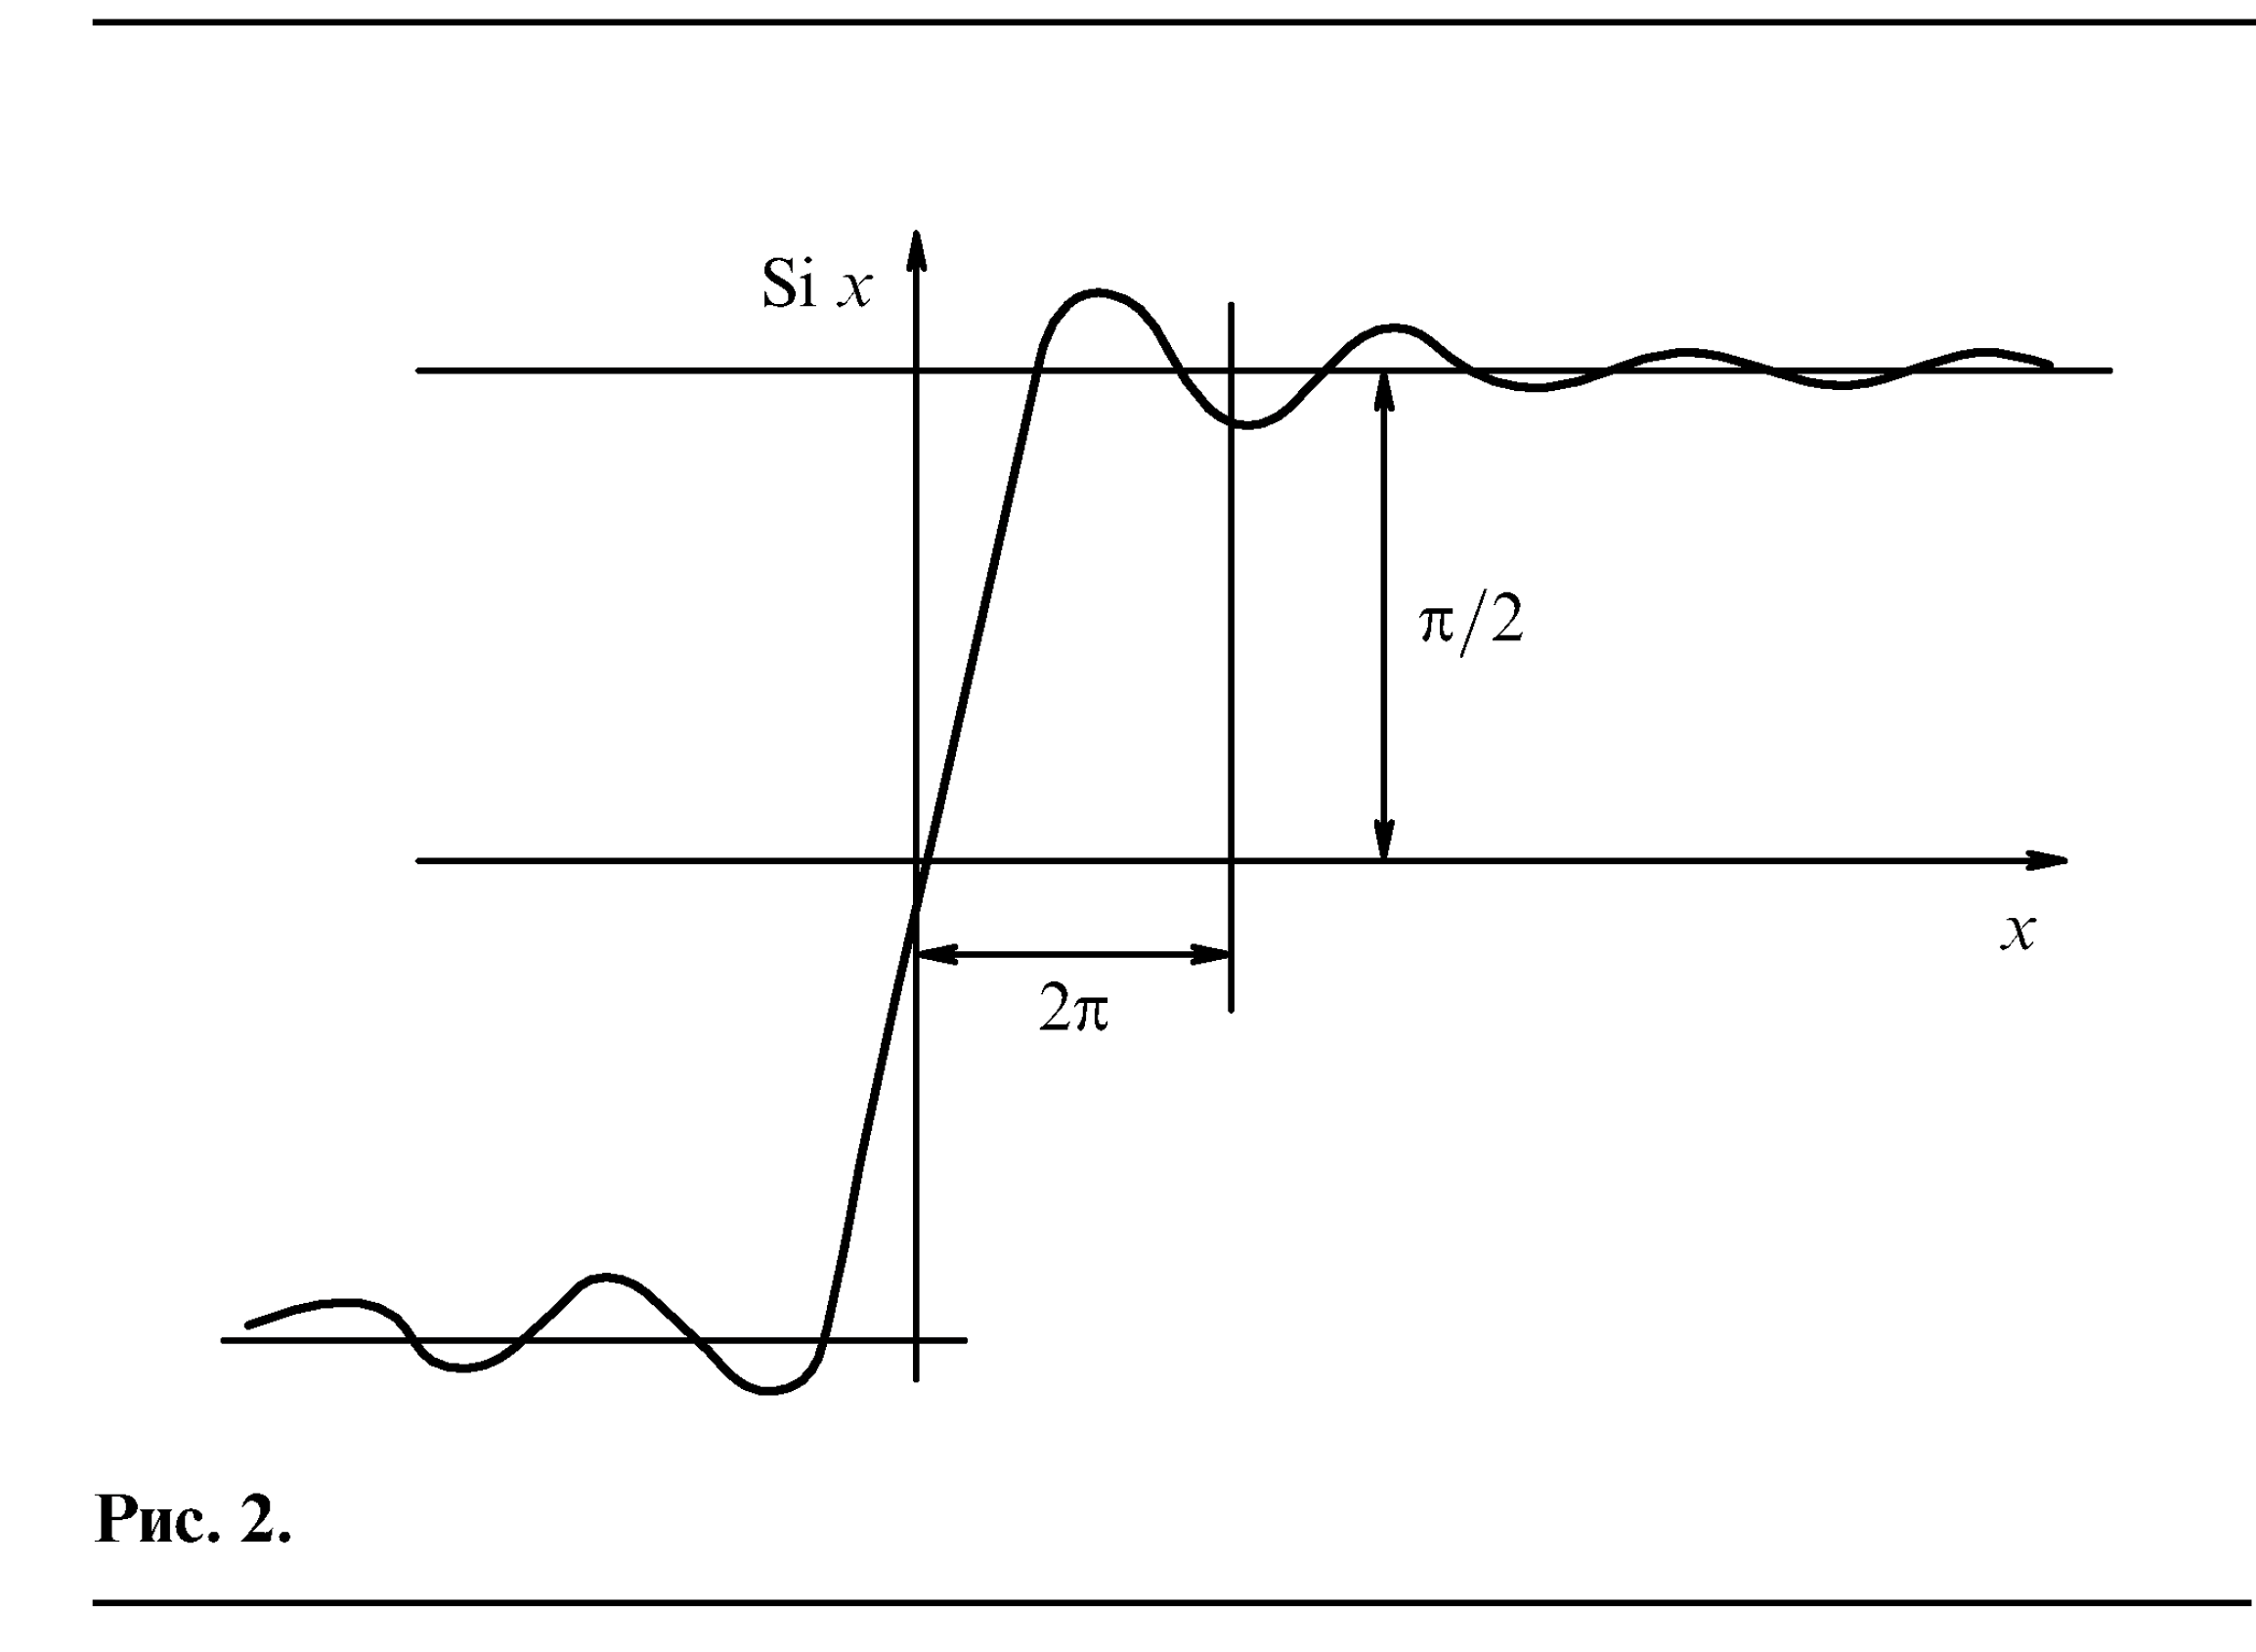
\includegraphics[width=0.7\linewidth]{bezianova_pic_2.png}
        \caption{~}
        \label{fig::bezianova_pic_2}
    \end{figure}

Как видно из рисунка, Si $x$ при $x \rightarrow \pm \infty$ стремится к $\pm \pi / 2$.

Рассмотрим значение квадратной скобки в выражении (\ref{bezianova_eq_11}). На рис.~\ref{fig::bezianova_pic_3а}(а) дано графическое изображение её при $T=3 /\left(2 f_1\right)$, на рис.~\ref{fig::bezianova_pic_3а}(б) --- при $T=6 /\left(2 f_1\right)$, на рис. \ref{fig::bezianova_pic_3а}(в) --- при $T=24 /\left(2 f_1\right)$ и на рис. \ref{fig::bezianova_pic_3а}(г) --- при $T=\infty$.

\begin{figure}[H]
        \centering
        \includegraphics[width=0.7\linewidth]{bezianova_pic_3а.png}
        \caption{~}
        \label{fig::bezianova_pic_3а}
    \end{figure}
Как видно из этих рисунков, квадратная скобка в выражении (\ref{bezianova_eq_11}) с увеличением $T$ стремится к пределам рис.~\ref{fig::bezianova_pic_3а}(г), т. е.
$$
\begin{array}{ll}
\text { при } \omega>\omega_1: & {[\text{ }]=0,} \\
\text { при } \omega<\omega_1: & {[\text{ }]=\pi .}
\end{array}
$$
\qquad Это также видно и непосредственно из выражения (\ref{bezianova_eq_11}), так как при увеличении $T$ увеличивается как бы масштаб при $\omega$ и Si делается очень быстро затухающим.

Таким образом, полученная сумма из $F_k(t)$ будет иметь амплитуды на частотах $f>f_1$ сколь угодно малыми, если взять $T$ достаточно большим.

По принятой функции $F(t)$ легко восстановить передаваемые числа $D_k$, так как при $t=n /\left(2 f_1\right)$ все члены равны нулю за исключением члена, для которого $k=n$, последний же равен $D_n \omega$. Поэтому
$$
F\left(\frac{n}{2 f_1}\right)=D_n \omega.
$$
\qquad Таким образом, мы из нашей функции, измеряя её значение при $t=k /\left(2 f_1\right)$, будем в состоянии получить через каждую $t=1 /\left(2 f_1\right)$-ю секунду значение нового $D_k$, в секунду же получим $N=2 f_1$ передаваемых чисел, что и требовалось доказать.
\end{proof}

\subsection*{Функции, состоящие из частот от $f_1$ до $f_2$} 

\qquad Докажем теорему.
\paragraph{}

\begin{theorem}\label{bezianova_theor_4} Любая функция $F(t)$, состоящая из частот от $f_1$ до $f_2$, может быть представлена так:
\begin{equation}\label{bezianova_eq_13}
	    F(t)=F_1(t) \cos \frac{\omega_2+\omega_1}{2} t+F_2(t) \sin \frac{\omega_2+\omega_1}{2} t,
\end{equation}

где $\omega_1=2 \pi f_1, \omega_2=2 \pi f_2$, а $F_1(t)$ и $F_2(t)$ есть некоторые функции, состоящие из частот от 0 до $f=\left(f_2-f_1\right) / 2$. Н наоборот: если в уравнении (\ref{bezianova_eq_13}) $F_1(t)$ и $F_2(t)$ есть любые функции, состоящие из частот от 0 до $f=\left(f_2-f_1\right) / 2$, то $F(t)$ состоит из частот от $f_1$ до $f_2$.
\end{theorem}

\begin{proof}
Если $F(t)$ состоит лишь из частот от $f_1$ до $f_2$, то, очевидно, $C(\omega)$ и $S(\omega)$ для такой функции могут быть представлены так:

\begin{equation}
	\begin{aligned}
	& C(\omega)=S(\omega)=0 \text { при } \omega>\omega_2 \text { или } \omega<\omega_1 \text {, } \\
	&\begin{rcases}
	C(\omega)=\sum_0^{\infty} A_k \cos \frac{\pi k}{2\left(\omega_2-\omega_1\right)}\left(\omega-\omega_1\right) \text{} \\
	S(\omega)=\sum_0^{\infty} B_k \sin \frac{\pi k}{2\left(\omega_2-\omega_1\right)}\left(\omega-\omega_1\right) \text{} \\
	\end{rcases}	
	\text { при } \omega_1<\omega<\omega_2, 
	\end{aligned}
\end{equation}


или, опять вводя обозначения (\ref{bezianova_eq_6}):

\begin{equation*}
\begin{gathered}
D_k=\frac{A_k+B_k}{2}, \\
D_{-k}=\frac{A_k-B_k}{2}, 
\end{gathered}
\end{equation*}

мы получим

\begin{equation}\label{bezianova_eq_14}
\begin{gathered}
\begin{rcases}
& C(\omega)=\sum_{-\infty}^{+\infty} D_k \cos \frac{\pi}{\omega_2-\omega_1} k\left(\omega-\omega_1\right) \\ 
& S(\omega)=\sum_{-\infty}^{+\infty} D_k \sin \frac{\pi}{\omega_2-\omega_1} k\left(\omega-\omega_1\right) \\ 
\end{rcases}
$$
\text { при } \omega_1<\omega<\omega_2. 
$$ \tag{14}
\end{gathered}
\end{equation}

\qquad Подставляя уравнения (\ref{bezianova_eq_14}) в уравнение (\ref{bezianova_eq_2}), мы получим после интегрирования и некоторого преобразования (см. приложение III):

\begin{equation}\label{bezianova_eq_15}
\begin{gathered}
 F(t)=\left[2 \sum_{-\infty}^{+\infty}(-1)^n D_{2 n} \frac{\sin \left(\omega_2-\omega_1\right) / 2\left\{t-k /\left(f_2-f_1\right)\right\}}{t-k /\left(f_2-f_1\right)}\right] \times \cos \frac{\omega_2+\omega_1}{2} t + \\
 + \left[2 \sum_{-\infty}^{+\infty}(-1)^n D_{2 n+1} \frac{\sin \left(\omega_2-\omega_1\right) / 2\left\{t-(k+1 / 2) /\left(f_2-f_1\right)\right\}}{t-(k+1 / 2) /\left(f_2-f_1\right)}\right] \times \sin \frac{\omega_2+\omega_1}{2} t, 
\end{gathered}
\end{equation}
или, обозначая

\begin{equation}\label{bezianova_eq_16}
\begin{gathered}
 F_1(t)=2 \sum_{-\infty}^{+\infty}(-1)^n D_{2 n} \times \frac{\sin \left(\omega_2-\omega_1\right) / 2\left[t-k /\left(f_2-f_1\right)\right]}{t-k /\left(f_2-f_1\right)}, 
\end{gathered}
\end{equation}

\begin{equation}\label{bezianova_eq_17}
\begin{gathered}
F_2(t)=2 \sum_{-\infty}^{+\infty}(-1)^n D_{2 n+1} \times \frac{\sin \left(\omega_2-\omega_1\right) / 2\left[t-(k+1 / 2) /\left(f_2-f_1\right)\right]}{t-(k+1 / 2) /\left(f_2-f_1\right)}, 
\end{gathered}
\end{equation}
и принимая во внимание, что согласно теореме~\ref{bezianova_theor_1} $F_1(t)$ и $F_2(t)$ должны обязательно состоять из спектра частот от 0 до $f=\left(f_2-f_1\right) / 2$, так как ряды (\ref{bezianova_eq_16}) и (\ref{bezianova_eq_17}) отличаются от ряда (\ref{bezianova_eq_1}) лишь обозначением, можно считать первую часть теоремы~\ref{bezianova_theor_4} доказанной.

Так как рядами (\ref{bezianova_eq_16}) и (\ref{bezianova_eq_17}) можно, согласно теореме~\ref{bezianova_theor_1}, представить любые функции $F_1(t)$ и $F_2(t)$, если они состоят из частот от 0 до $f=\left(f_2-f_1\right) / 2$, и так как на коэффициенты $D_k$, входящие в эти ряды, не наложены никакие условия, то, очевидно, верна и вторая часть теоремы~\ref{bezianova_theor_4}.
\end{proof}

Докажем теперь две теоремы, которые являются обобщением теорем~\ref{bezianova_theor_2} и~\ref{bezianova_theor_3}.
\paragraph{}

\begin{theorem}\label{bezianova_theor_5} Любую функцию $F(t)$, состоящую из частот от $f_1$ до $f_2$, можно непрерывно передавать с любой точностью при помощи чисел, передаваемых друг за другом через $1 /\left[2\left(f_2-f_1\right)\right]$ секунд.
	\end{theorem}

\begin{proof}
Действительно, при $t=k /\left(f_2+f_1\right)(k-$ целое число) мы согласно формуле (\ref{bezianova_eq_13}) получим:
\begin{equation}\label{bezianova_eq_18}
\begin{gathered}
F\left(\frac{k}{f_2+f_1}\right)=F_1\left(\frac{k}{f_2+f_1}\right),
\end{gathered}
\end{equation}
так как при этом значении $t$ косинус равен 1 , а синус --- 0 . Когда же $t=(k+1 / 2) /\left(f_2+f_1\right)$, мы получим
$$
F\left(\frac{k+1 / 2}{f_2+f_1}\right)=F_2\left(\frac{k+1 / 2}{f_2+f_1}\right)
$$
по аналогичным соображениям.

Таким образом, через каждую $1 /\left(f_2+f_1\right)$-ю секунду мы будем в состоянии узнавать по одному значению $F_1(t)$ и $F_2(t)$, по этим значениям мы сможем воспроизводить и сами функции $F_1(t)$ и $F_2(t)$, так как согласно теореме~\ref{bezianova_theor_2} по так часто следующим числам можно воспроизводить функции, состоящие из частот от 0 до $\left(f_2+f_1\right) / 2$, функции же $F_1(t)$ и $F_2(t)$ состоят лишь из частот от 0 до $\left(f_2-f_1\right) / 2$.

Каждую из полученных таким образом функций можно как состоящую из частот 0 до $\left(f_2-f_1\right) / 2$ передавать, согласно теореме~\ref{bezianova_theor_2}, числами, следующими друг за другом через $1 /\left(f_2-f_1\right)$ секунд, а эти две функции одновременно можно передавать, очевидно, числами, следующими друг за другом через $1 /\left[2\left(f_2-f_1\right)\right]$ секунд, по этим числам восстанавливая сначала $F_1(t)$ и $F_2(t)$, мы по ним сможем по формуле (\ref{bezianova_eq_13}) восстановить и саму $F(t)$.
\end{proof}

\begin{theorem}\label{bezianova_theor_6} Можно непрерывно и равномерно передавать произвольные числа $D_k$ со скоростью $N$ чисел в секунду при помощи функции $F(t)$, имеющей слагаемые на частотах $f>f_2$ и $f<f_1$ сколь угодно малыми (т. е. практически их не имеющей), если
\begin{equation} \label{bezianova_eq_19}
\begin{gathered}
N=2\left(f_2-f_1\right). 
\end{gathered}
\end{equation}
\end{theorem}

\begin{proof}
Действительно, мы можем передавать согласно теореме~\ref{bezianova_theor_3} $N$ чисел в секунду при помощи двух функций $F_1(t)$ и $F_2(t)$, причем каждая будет иметь слагаемые на частотах выше $\left(f_2-f_1\right) / 2$ сколь угодно малыми.

Эти же функции можно непрерывно передавать функцией $F(t)$, имеющей слагаемые на частотах $f>f_2$ и $f<f_1$ сколь угодно малыми. Действительно, по функциям $F_1(t)$ и $F_2(t)$ согласно уравнению (\ref{bezianova_eq_13}) мы получим $F(t)$, передавая которую, мы, как указывалось выше, сможем по ней восстанавливать $F_1(t)$ и $F_2(t)$, а по ним и передаваемые числа.
\end{proof}
Для доказательства последней теоремы, в которой будет говориться о невозможности передавать при помощи функции, состоящей из ограниченного диапазона частот, беспредельно многого, докажем следующую лемму.

\paragraph{}

\begin{lemma}\label{bezianova_lemma_1} Нельзя при помощи $M$ чисел передавать $N$ произвольных чисел, если
\begin{equation}\label{bezianova_eq_20}
\begin{gathered}
M<N. 
\end{gathered}
\end{equation}
\end{lemma}

\begin{proof}
Предположим, что это сделать можно.
Тогда, очевидно, $M$ чисел $m_1, \ldots, m_M$ есть какие-то функции $N$ чисел $n_1, \ldots, n_N$, т. е.

\begin{equation}\label{bezianova_eq_21}
\begin{gathered}
m_1=\varphi_1\left(n_1, \ldots, n_N\right), \\
m_2=\varphi_2\left(n_1, \ldots, n_N\right), \\
\ldots\ldots\ldots\ldots\ldots\ldots \\
m_M=\varphi_M\left(n_1, \ldots, n_N\right), 
\end{gathered}
\end{equation}
и мы, очевидно, должны, зная лишь $M$ чисел $m_1, \ldots, m_M$ и, конечно, зная функции $\varphi_1, \ldots, \varphi_M$, суметь восстановить по ним числа $n_1, \ldots, n_N$.

Но это равносильно решению $M$ уравнений (\ref{bezianova_eq_21}) с $N$ неизвестными, что сделать невозможно, если уравнений меньше, чем неизвестных, т. е. справедливо неравенство (\ref{bezianova_eq_20}).
\end{proof}
\paragraph{}

\begin{theorem}\label{bezianova_theor_7} Можно непрерывно передавать произвольные, следующие друг за другом равномерно числа со скоростью $N$ чисел в секунду и $M$ произвольных функций $F_1(t), \ldots, F_M(t)$ с диапазонами частот шириной $\Delta f_1, \ldots, \Delta f_M$ при помощи непрерывно следующих друг за другом чисел со скоростью $N^{\prime}$ чисел в секунду и при помощи $M^{\prime}$ функций $F_1^{\prime}(t), \ldots, F_{M^{\prime}}^{\prime}(t)$ с диапазонами частот $\Delta f_1^{\prime}, \ldots, \Delta f_{M^{\prime}}^{\prime}$, если
\begin{equation}\label{bezianova_eq_22}
\begin{gathered}
N+2 \sum_1^M \Delta f_k \leqslant N^{\prime}+2 \sum_1^{M^{\prime}} \Delta f_k^{\prime}.
\end{gathered}
\end{equation}
И это никаким образом сделать нельзя, если
\begin{equation}\label{bezianova_eq_23}
\begin{gathered}
N+2 \sum_1^M \Delta f_k>N^{\prime}+2 \sum_1^{M^{\prime}} \Delta f_k^{\prime}.
\end{gathered}
\end{equation}
\end{theorem}

\begin{proof}
Первая часть этой теоремы доказывается на основании теорем~\ref{bezianova_theor_5} и~\ref{bezianova_theor_6}.

Действительно, на основании теоремы $\mathrm{V}$ мы можем передавать наши $N$ чисел в секунду и $M$ кривых при помощи $P$ чисел в секунду, если
\begin{equation}\label{bezianova_eq_24}
\begin{gathered}
P=N+2 \sum_I^M \Delta f_k.
\end{gathered}
\end{equation}

А эти $P$ чисел в секунду можно отчасти передавать при помощи $N^{\prime}$ чисел в секунду, а отчасти по теореме~\ref{bezianova_theor_6} при помощи кривых $F_1^{\prime}(t), \ldots, F_{M^{\prime}}^{\prime}(t)$, если справедливо равенство (\ref{bezianova_eq_22}).

Вторую часть теоремы докажем от противного, исходя из леммы.

Пусть нам нужно передавать $P$ произвольных чисел в секунду, это по теореме~\ref{bezianova_theor_6} можно сделать, передавая $N$ чисел в секунду и функции $F_1(t), \ldots, F_M(t)$ с диапазонами частот $\Delta f_1, \ldots, \Delta f_M$, если справедливо равенство (\ref{bezianova_eq_24}).

А эти функции и числа, если была бы несправедлива вторая часть теоремы, можно было бы передавать при помощи функций $F_1^{\prime}(t), \ldots, F_{M^{\prime}}^{\prime}(t)$ и $N^{\prime}$ чисел в секунду. Последние же числа и функции можно согласно теореме~\ref{bezianova_theor_5} передавать при помощи $P^{\prime}$ чисел в секунду, если
\begin{equation}\label{bezianova_eq_25}
\begin{gathered}
P^{\prime}=N^{\prime}+2 \sum_1^{M^{\prime}} \Delta f_k^{\prime}. 
\end{gathered}
\end{equation}

Другими словами, мы смогли бы непрерывно передавать $P$ чисел в секунду при помощи $P^{\prime}$ чисел в секунду, хотя согласно равенствам (\ref{bezianova_eq_24}) и (\ref{bezianova_eq_25}) и неравенству (\ref{bezianova_eq_23})
$$
P>P^{\prime} \text {. }
$$

Таким образом, предположение, что вторая часть теоремы~\ref{bezianova_theor_7} не верна, приводит нас к недопустимому, согласно доказанной лемме, результату.
\end{proof}

\subsection*{Пропускная способность при телефонной передаче}
\qquad Разговор, музыка и другие объекты телефонной передачи являются произвольными функциями времени, состоящими из спектра частот, ширина которого вполне определённа и зависит от того, насколько полно мы хотим передавать звук.

Передавая эту функцию по проволоке или по радио, мы превращаем её в другую функцию времени, которую собственно уже и передаём. Причём эта последняя функция должна обязательно, согласно теореме~\ref{bezianova_theor_7}, при непрерывной передаче иметь спектр частот шириной не меньшей, чем та полоса звуковых частот, которую мы хотим передать.

Таким образом, непрерывная телефонная передача не может занимать в эфире или в проволоке меньший диапазон частот, чем ширина спектра звуковых частот, требуемая для данной передачи. Это верно вне зависимости от способа передачи, и нельзя выдумать такого способа, который позволил бы занять при непрерывной передаче более узкий диапазон частот.

Такой минимальный спектр частот, как известно, может дать уже в настоящее время передача на одной боковой полосе.

Оговорка «при непрерывной передаче» имеет большое значение, так как можно, передавая с перерывами какие-нибудь звуки, скажем, музыку, занимать меньший диапазон частот, чем ширина звукового спектра, которую мы при этом будем получать. Для этого достаточно записывать передаваемую музыку сначала на граммофонные пластинки, а затем передавать с них, вращая, скажем, вдвое медленнее, чем при записи. Тогда все частоты будут получаться вдвое меньше нормального и мы при передаче сумеем занять вдвое меньший диапазон частот. Восстанавливать такую передачу можно также посредством граммофона. Ясно, что такая передача не может увеличить пропускную способность, так как при ней «эфир» или проволока будут заняты все время, а передача будет идти с перерывамн.

Это также не противоречит и теореме~\ref{bezianova_theor_7}, так как там оговорено: «произольную функцию» и «непрерывно» нельзя передавать, а прн такой передаче мы можем передавать или с перерывами произвольную функцию, нли беспрерывно функцию не совсем произвольную, а имеющую уже известные перерывы.

Из теоремы~\ref{bezianova_theor_7} также следует, что нельзя увеличить пропускную способность путём применения каких-нибудь селекций не частотного характера (не касаясь направленных антенн) нли еще чем-нибудь подобным.

Действительно, если бы это можно было бы сделать, то, применяя эти способы, можно было бы с одного места передавать в другое, скажем, $n$ телефонных передач одновременно со спектрами частот шириной $\Delta f$ каждая, занимая для этого диапазон частот, меньший, чем $n \Delta f$.

Но при такой передаче напряжённости поля (или токи в проволоке) oт разных передач смешались бы в одну какую-то функцию времени co спектрами частот меньших $n \Delta f$, которая и будет восприниматься приемниками. Получится, что мы смогли передать $n$ функций времени с диапазонами частот шириной $\Delta f$ при помощи одной функции с диапазоном частот, меньшим, чем $n \Delta f$, что, согласно теореме~\ref{bezianova_theor_7}, совершенно невозможно.

Из сказанного ясно, что для телефона увеличить пропускную способность эфнра можно, лишь применяя направленные антенны нли расширяя эксплуатируемый диапазон частот путём использования ультракоротких волн.

\subsection*{Передача изображений и телевидение со всеми полутенями}

\qquad При передаче изображений и телевидении нужно передавать степень черноты каких-то $N$ элементов в секунду, а это равноснльно передаче произвольных чисел со скоростью $N$ чисел в секунду. Если мы это хотим сделать при помощи функции времени, как это всегда и делается, то по теореме~\ref{bezianova_theor_7} она должна занять диапазон частот, не меньший, чем $N / 2$ периодов в секунду. Таким образом, сразу видно, что полосу частот и тут сократить нельзя больше, чем это позволяет сделать передача на одной боковой полосе. Правда, для осуществления и этого могут встретиться большие технические трудности из-за фазовых искажений, возможных при такой передаче.

Нельзя сократить полосу частот и при помощи какой-нибудь «групповой развертки изображений» (развёртке не по отдельным элементам), так как и при такой развёртке придется всё же передать, правда, каким-то другим способом, степень почернения тех же $N$ элементов в секунду, т. е. $N$ произвольных чисел в секунду, что сделать никак с уменьшенным диапазоном частот нельзя.

Не смогут и тут помочь нечастотные методы селекции (не включая направленных антенн) по тем же основаниям, как и при телефонной nередаче.

\subsection*{Телеграфная передача и передача изображений без полутеней или с ограниченным количеством их}

\qquad При телеграфной передаче, а также при передаче изображений без полутеней нли с вполне определёнными заранее известными полутенями, мы имеем дело опять с передачей каких-то $N$ элементов в секунду, что равносильно передаче $N$ чисел в секунду, но величина этих элементов и, значит, чисел не может быть вполне произвольной, a должна иметь вполне определеннье, наперёд известнье значения. Поэтому к этим передачам нельзя прямо применять выше выведенные теоремы, так как там говорится о передаче произвольных, наперёд совершенно неизвестных чисел.

Действительно, для этих передач можно сократить необходимый диапазон частот во сколько угодно раз, а следовательно, по крайней мере теоретически, увеличить пропускную способность также в любое число раз.

Для этого можно поступать таким образом: скажем, мы хотим передавать со скоростью $N$ элементов в секунду элементы, которые могут иметь значение либо 0, либо 1, и занять для этого диапазон частот всето лишь шириной $N / 4$ (вместо $N / 2$ по теореме~\ref{bezianova_theor_7}). Для этого будем передавать два таких элемента посредством одного элемента (или числа), хотя бы согласно следующей таблице, где в графе I дано значение первого элемента, в графе II --- второго, а в графе III --- значение элемента, которому мы хотим их передать.

\begin{figure}[H]
        \centering
        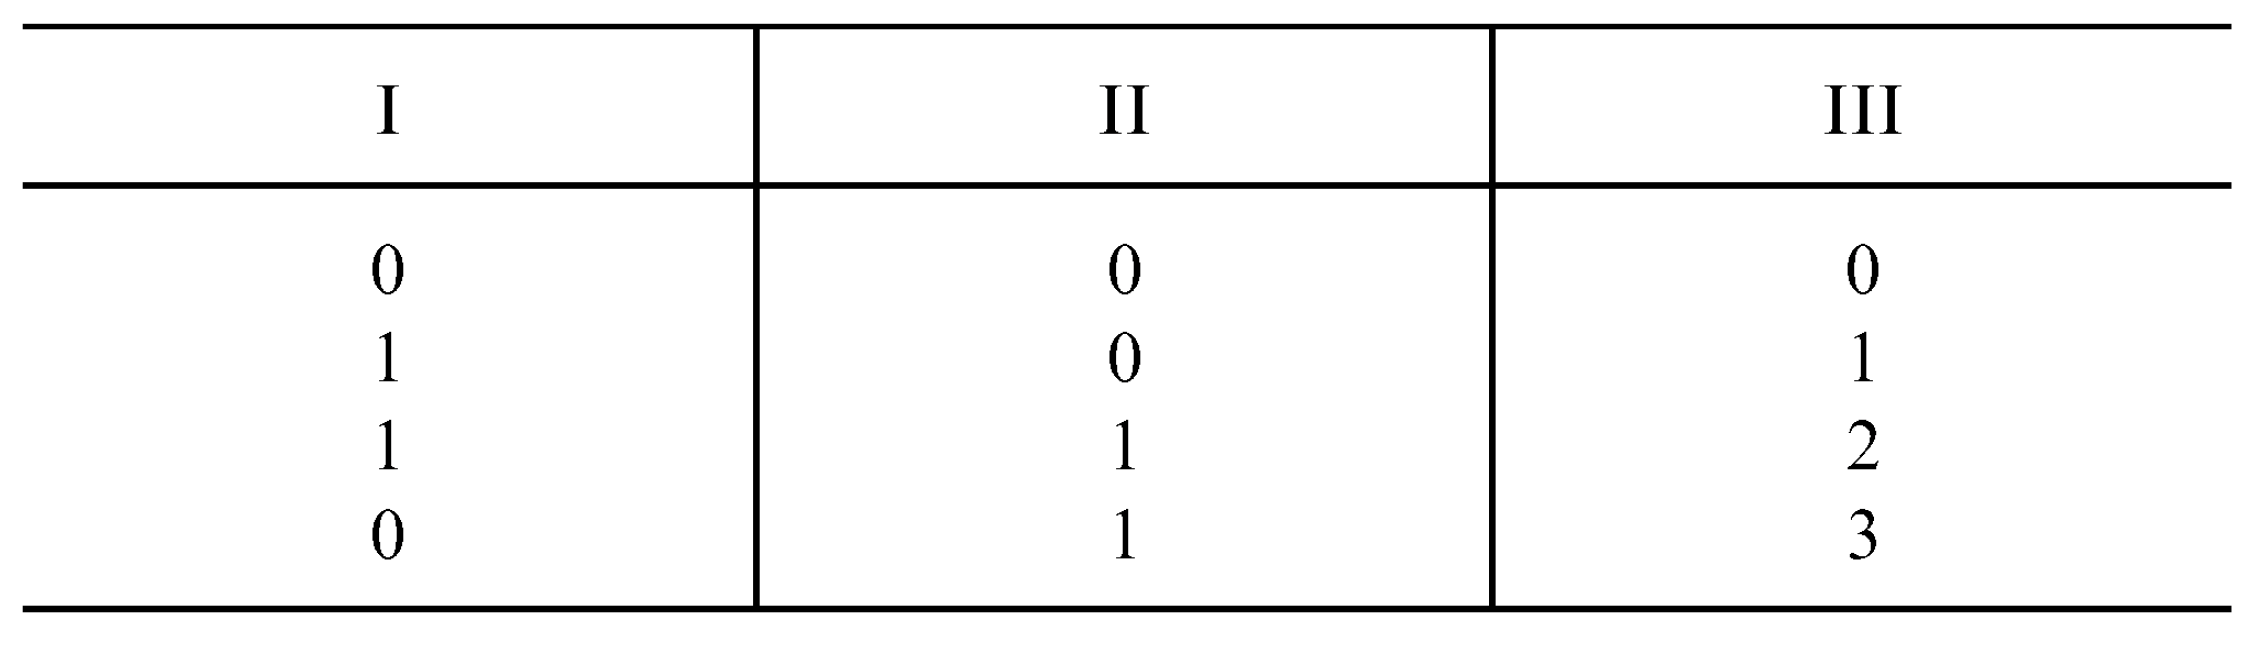
\includegraphics[width=0.7\linewidth]{bezianova_fig_1.png}
        \caption{~}
        \label{fig::bezianova_fig_1}
    \end{figure}

Таким образом мы сможем передавать $\mathrm{N}$ элементов в секунду, имеющих по два значения, при помощи $N / 2$ элементов в секунду, могущих иметь по 4 значения, которые, согласно теореме~\ref{bezianova_theor_7}, могут передаваться при помощи диапазона частот шириной $N / 4$.

Практически такую замену двух элементов одним можно осуществить хотя бы по cхеме рис. 4, где $\Phi_1$ и $\Phi_2$ --- два фотоэлемента или два телеграфных аппарата, причём $\Phi_1$ приводит в действие модулятор $\mathrm{M}_1$, посылающнй в линию амплитуду, равную единице, $\Phi_2$ же работает с модулятором $\mathrm{M}_2$, посылающим амплитуду, равную 3. При работе $\Phi_1$ и $\Phi_2$ сразу приводятся в действие оба модулятора, и так как они включены навстречу, то посылается амплитуда, равная 2. На приём принимаемый сигнал поступает на три приёмника, причём первый, $\Pi_1$, начинает работать от амплитуды 1 , второй, $\Pi_2$, --- от амплитуды 2 и третий, $\Pi_3$, --- от амплитуды 3. Первый приёмник $\Pi_1$ приводит в действие $\text{Л}_1$, второй --- $\text{Л}_2$, а третий при приходе амплитуды, равной трём, --- запирает доступ от 1 приёмника на $\text{Л}_1$. При помощи такой схемы мы получим указанное выше сокращение полосы частот.

\begin{figure}[H]
        \centering
        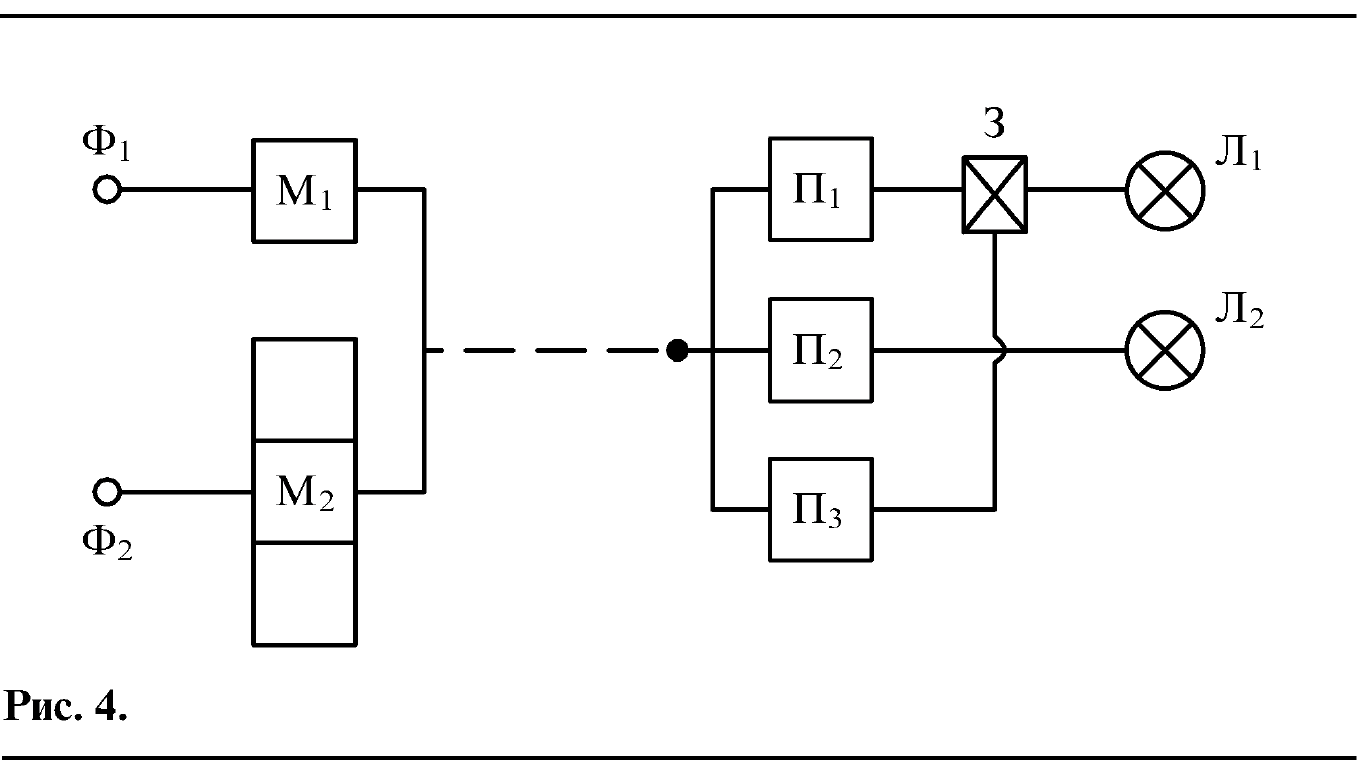
\includegraphics[width=0.7\linewidth]{bezianova_pic_4.png}
        \caption{~}
        \label{fig::bezianova_pic_4}
    \end{figure}

При такой передаче ввиду того, что при ней становится необходимым различать вместо двух четыре градации принимаемых сигналов, необходимо, очевидно, будет увеличить мощность передатчика в $3^2=9$ раз, по сравнению с обычной передачей.

Возможно сократить аналогичным образом полосу частот и в $n$ раз, передавая $n$ элементов, могущих иметь по два значения, при помощи одного элемента, который должен для этого, очевидно, иметь $2^n$ значений (по числу комбинаций из $n$ элементов, имеющих по два значения). Но для такой передачи необходимо увеличение мощности в $\left(2^n-1\right)^2$ раз.

При передаче изображений с опредёленным количеством заданных наперёд полутеней каждый элемент должен иметь несколько, скажем $m$ (для этого случая $m>2$), значений. Для сокращения полосы частот при такой передаче в $n$ раз можно заменить $n$ передаваемых элементов одним, который должен иметь возможность принимать $m^n$ значений (по числу возможных комбинаций из $n$ элементов, имеющих $m$ возможных значений каждый). Мощность при этом, очевидно, необходимо будет увеличить в $\left[\left(m^n-1\right)^2\right] /\left[(m-1)^2\right]$ раз.

Как видно, такое уменьшение полосы частот требует колоссального увеличения мощности.

Кроме того, приведённые здесь способы будут очень плохи при передаче на коротких волнах из-за фадингов.

Для проволочной связи уменьшение таким способом полосы частот может иметь практическое значение уже и сейчас, так как мощности, там необходимые, малы и нет быстрых изменений силы приёма.

\subsection*{Приложение I}

\qquad Подставляя выражение (\ref{bezianova_eq_7}) в уравнение (\ref{bezianova_eq_4}), мы получим:
$$
\begin{aligned}
& F(t)=\int_0^{\omega_1} \sum_{-\infty}^{+\infty} D_k \cos \frac{\pi}{\omega_1} k \omega \cos \omega t \text{ d} \omega+\int_0^{\omega_1} \sum_{-\infty}^{+\infty} D_k \sin \frac{\pi}{\omega_1} k \omega \sin \omega t \text{ d} \omega= \\
& =\sum_{-\infty}^{+\infty} D_k \int_0^{\omega_1}\left(\cos \frac{\pi}{\omega_1} k \omega \cos \omega t+\sin \frac{\pi}{\omega_1} k \omega \sin \omega t\right) \text{ d} \omega= \\
& =\sum_{-\infty}^{+\infty} D_k \int_0^{\omega_1}\left(\cos \left(t-\frac{\pi}{\omega_1} k\right)\right) \text{ d} \omega, \\
&
\end{aligned}
$$
или, интегрируя и заменяя в круглой скобке $\omega_1$ на $2 \pi f_1$, получнм
$$
F(t)=\sum_{-\infty}^{+\infty} D_k \frac{\sin \omega_1 \left(t-k /\left(2 f_1\right)\right)}{t-k /\left(2 f_1\right)} \text {. }
$$

\subsection*{Приложение II}

\qquad B
$$
C(\omega)=\frac{1}{\pi} \int_{k /\left(2 f_1\right)-T}^{k /\left(2 f_1\right)+T} D_k \frac{\sin \omega_1\left(t-k /\left(2 f_1\right)\right)}{t-k /\left(2 f_1\right)} \cos \omega t \text{ d} t
$$
сделаем подстановку
$$
t=u+\frac{k}{2 f_1}, \quad \text{ d} t = \text{ d} u,
$$
тогда
$$
\begin{aligned}
C(\omega) & =\frac{1}{\pi} \int_{-T}^T D_k \frac{\sin \omega_1 u}{u} \cos \omega\left(u+\frac{k}{2 f_1}\right) \text{ d} u= \\
& =\frac{1}{\pi} \int_{-T}^T D_k \frac{\sin \omega_1 u \cos \omega u}{u} \cos \omega \frac{k}{2 f_1} \text{ d} u+\frac{1}{\pi} \int_{-T}^T D_k \frac{\sin \omega_1 u \sin \omega u}{u} \sin \omega \frac{k}{2 f_1} \text{ d} u .
\end{aligned}
$$

Функция, стоящая под вторым интегралом, при переходе через нуль меняет свой знак, оставаясь по величине той же, поэтому второй интеграл равен нулю.

Функция же под первым интегралом не меняется при замене $u$ на $-u$, и поэтому пределы этого интеграла можно взять от 0 до $T$, помножив при этом ннтеграл на два. Значит,
$$
C(\omega)=\frac{2 D_k}{\pi} \cos \omega \frac{k}{2 f_1} \int_0^T \frac{\sin \omega_1 u \cos \omega u}{u} \text{ d} u
$$
или
$$
C(\omega)=\frac{D_k}{\pi} \cos \omega \frac{k}{2 f_1}\left[\int_0^T \frac{\sin \left(\omega_1+\omega\right) u}{u} \text{ d} u-\int_0^T \frac{\sin \left(\omega-\omega_1\right) u}{u} \text{ d} u\right] .
$$
Заменяя в первом интеграле
$$
\left(w_1+\omega\right) u=y,
$$
a во втором
$$
\left(w-\omega_1\right) u=y,
$$
получим
$$
C(\omega)=\frac{D_k}{\pi} \cos \omega \frac{k}{2 f_1}\left[\int_0^{\left(\omega+\omega_1\right) T} \frac{\sin y}{y} \text{ d} y-\int_0^{\left(\omega-\omega_1\right) T} \frac{\sin y}{y} \text{ d} y\right] .
$$

Стоящие в скобках интегралы не берутся. Это, очевидно, будут какие-то функции верхнего предела. Прннято эти функции называть ннтегральными синусами. Введя это понятие, получнм:
$$
C(\omega)=\frac{D_k}{\pi} \cos \omega \frac{k}{2 f_1}\left[\operatorname{Si} T\left(\omega+\omega_1\right)-\operatorname{Si} T\left(\omega-\omega_1\right)\right] .
$$
Проделывая совершенно то же с $S(\omega)$, мы получим уравнение (\ref{bezianova_eq_11}).

\subsection*{Приложение III}

\qquad Подставляя уравнения (\ref{bezianova_eq_14}) в уравнение \ref{bezianova_eq_2}, получим
$$
F(t)=\int_{\omega_1}^{\omega_2} \sum_{-\infty}^{+\infty} D_k \cos \frac{\pi k\left(\omega-\omega_1\right)}{\omega_2-\omega_1} \cos \omega t \text{ d} \omega+\int_{\omega_1}^{\omega_1} \sum_{-\infty}^{+\infty} D_k \sin \frac{\pi k\left(\omega-\omega_1\right)}{\omega_2-\omega_1} \sin \omega t \text{ d} \omega.
$$
Пределы взяты от $\omega_1$ и $\omega_2$, потому что
$$
C(\omega)=S(\omega)=0
$$
прн
$$
\omega<\omega_1 \quad \text { или } \quad \omega>\omega_2 .
$$

После тригонометрических преооразований
$$
\begin{aligned}
& F(t)=\sum_{-\infty}^{+\infty} D_k \times \int_{\omega_1}^{\omega_2} \cos \left[\omega\left(t-\frac{\pi k}{\omega_2-\omega_1}\right)+\frac{\pi k \omega_1}{\omega_2-\omega_1}\right] \text{ d} \omega= \\
&=\sum_{-\infty}^{+\infty} D_k \times \frac{\sin \left[\omega_2\left[t-\pi k /\left(\omega_2-\omega_1\right)\right]+\pi k \omega_1 /\left(\omega_2-\omega_1\right)\right]}{t-\pi k /\left(\omega_2-\omega_1\right)}- \\
&-\frac{\sin \left[\omega_1\left[t-\pi k /\left(\omega_2-\omega_1\right)\right]+\pi k \omega_1 /\left(\omega_2-\omega_1\right)\right]}{t-\pi k /\left(\omega_2-\omega_1\right)} .
\end{aligned}
$$
Заменяя разность синусов на произведение и произведя упрощения, nолучим:
$$
F(t)=2 \sum_{-\infty}^{+\infty} D_k \times \cos \left(\frac{\omega_2+\omega_1}{2} t-\frac{\pi}{2} k\right) \times \frac{\sin \left[\left(\omega_2-\omega_1\right) / 2\left\{t-k /\left[2\left(f_2-f_1\right)\right]\right\}\right]}{t-k /\left[2\left(f_2-f_1\right)\right]},
$$
или, группируя члены с чётными и нечётными $k$ вместе, получим уравнение (\ref{bezianova_eq_15}).

\subsection*{Выводы}

\qquad 1) Ввиду имеющейся уже в настоящее время «тесноты в эфире» и в связи с дальнейшим бурным развитием радиотехники, в особенности с развитием коротковолновых телефонных передач и передач изображений, вопрос об изыскании способов увеличения пропускной способности эфира должеи быть поставлен перед научно-исследовательскими институтами во всей остроте.

Вопрос об увеличении пропускной способности проволоки имеет также большое экономическое значенне. Поэтому этот вопрос слепует тоже изучать.

2) Так как нельзя никакими способами, как, например, сужением полосы частот отдельных передач, применением каких-либо методов для разделения передач с накладывающимися друг на друга частотами и т. п., увеличить пропускную способность эфира или проволоки при передаче изображений и телефона больше, чем это позволяет сделать обычная передача с одной боковой полосой, то все попытки в этих направлениях следует оставить как неосуществимые.

3) Для телеграфа и передачи изображений без полутеней или с ограниченным количеством их пропускную способность можно теоретически повысить беспредельно, но это связано с большим увеличением мощности и усложнением аппаратуры. Поэтому надо думать, что такое сужение полосы частот может в ближайшее время найти применение лишь в проволочной связи, где над этим вопросом следует работать.

4) Необходимо для первой категории передач (телефон и передача изображений с полутенями) направить все усилия на разработку методов приёма и передачи на одной боковой полосе как методов, позволяющих максимально возможно использовать эфир и проволоку. 

Цель разработки --- усовершенствовать и упростить аппаратуру, очень сложную в настоящее время.

5) Необходимо изучить вопрос об увеличении пропускной способности эфира при помощи направленных антенн как приёмных, так и передающих.

6) Необходимо увеличить диапазон эксплуатируемых в эфире частот путём загрузки, где возможно, ультракоротких волн, а также изучением этого диапазона частот.

7) Необходимо изучать вопрос об увеличении стабильности частоты радиостанций, что позволит уплотнить эфир.

